% Réplica de Basso et al. (2026): resultados frente al paper.
% Compilar con:  latexmk -pdf -interaction=nonstopmode presentacion.tex
% Antes, si cambiaron los resultados:  .venv/Scripts/python.exe entregables/replica_vs_paper/generar_tablas.py
% Las figuras del paper (FiguraN_paperOriginal.png) están en figuras/ y no se versionan.
\documentclass[aspectratio=169,10pt,t]{beamer}
\usepackage[utf8]{inputenc}
\usepackage[T1]{fontenc}
\usepackage[spanish]{babel}
\usepackage{graphicx}
\usepackage{booktabs}
\usepackage{amssymb}
\usepackage[backend=biber,style=authoryear]{biblatex}
\addbibresource{../referencias.bib}

\graphicspath{{../../docs/figures/}{figuras/}}

% Estilo sobrio: fondo blanco, sin símbolos de navegación, solo el número de diapositiva.
\usetheme{default}
\setbeamertemplate{navigation symbols}{}
\setbeamertemplate{footline}{\hfill\insertframenumber\hspace{0.6cm}\vspace{0.3cm}}
\setbeamerfont{frametitle}{size=\large}

\title{Réplica Exposure to last-mile delivery emissions: A novel data fusion
approach TRD}
\subtitle{Basso et al.\ (2026)}
\author{Nicolás Fuentes}
\date{\today}

\begin{document}

\begin{frame}
  \titlepage
\end{frame}

% ------------------------------------------------------------------------------------------------
\begin{frame}{Qué hace el paper}
  \begin{itemize}
    \item Cruza, en una grilla \textbf{hexágono H3 (res.\ 9) $\times$ hora} (7--22 h), los vehículos de reparto (GPS de SimpliRoute) con la \textbf{composición demográfica de la población presente} (móviles de Entel).
    \item Pregunta: ¿qué grupos \emph{coinciden} más con los camiones de reparto? Mide co-ocurrencia, no concentraciones ni dosis.
    \item Modelos: \textbf{ZINB} para el conteo de vehículos y \textbf{OLS} para la distancia recorrida (tres especificaciones), con errores estándar agrupados por comuna (51 comunas).
    \item Compara el enfoque \textbf{dinámico} (población presente en cada hora) con el \textbf{estático} (composición residencial fija).
    \item 178.304 filas (11.144 hexágonos $\times$ 16 horas), miércoles de 2024 \parencite{basso2026}.
  \end{itemize}
\end{frame}

\begin{frame}{Cómo replicamos}
  \begin{itemize}
    \item \textbf{Datos:} el paquete de replicación de los autores: paneles finales y archivos diarios de conteos y distancias. No viene incluso \textbf{el GPS crudo} ni \textbf{los datos de Entel}: es reproducibilidad computacional, no una réplica independiente.
    \item Se replica \textbf{tal cual describe el paper}, incluidas decisiones que el paper no describe.
  \end{itemize}
\end{frame}

\begin{frame}{Resumen}
  \begin{columns}[T]
    \column{0.52\textwidth}
    \textbf{Coincide}
    \footnotesize
    \begin{itemize}
      \item Tabla 2: media, desviación y porcentajes (62/62 celdas)
      \item Tablas 4 y 5: valores (104/104 celdas, dentro del redondeo impreso)
      \item Medianas de conteos (42 miércoles) y de distancia y tiempo (41): idénticas
      \item Estrellas frente a las tablas regeneradas por los autores: 88/88
      \item Cameron--Trivedi: 7,750 frente a 7,73
      \item Figs.\ 6, 8, 9 y 10: mismos puntos
      \item Fig.\ 7: 12/12 etiquetas (con un factor derivado de ellas)
    \end{itemize}
    \column{0.46\textwidth}
    \textbf{Difiere}
    \footnotesize
    \begin{itemize}
      \item Estrellas \emph{impresas}: 23/44 (Tabla 4) y 38/44 (Tabla 5)
      \item I de Moran: 0,419 y 0,430 frente a 0,4694 y 0,4756
      \item Wasserstein: 13 de 15 valores dentro de la banda del 95\,\%
      \item Fig.\ 1: escalas de color 1.511 y 7.073 frente a 1.600 y 7.000
      \item Fig.\ 2 y Tabla 3: necesitan el GPS crudo (sustituto)
    \end{itemize}
  \end{columns}
\end{frame}

% ------------------------------------------------------------------------------------------------
\section{Lo que coincide}

\begin{frame}{Tabla 2: población flotante (media y desviación)}
  \centering\footnotesize
  \begin{tabular}{lrrrr}\toprule
 & \multicolumn{2}{c}{Media} & \multicolumn{2}{c}{Desviación} \\
Variable & Réplica & Paper & Réplica & Paper \\\midrule
Avg Population & 472,78 & 472,78 & 938,57 & 938,57 \\
Male & 232,93 & 232,93 & 464,99 & 464,99 \\
Female & 239,83 & 239,83 & 474,95 & 474,95 \\
Under 25 & 81,74 & 81,74 & 147,03 & 147,03 \\
25-34 & 85,80 & 85,80 & 193,85 & 193,85 \\
35-44 & 91,61 & 91,61 & 195,21 & 195,21 \\
45-54 & 87,63 & 87,63 & 177,84 & 177,84 \\
55-64 & 70,70 & 70,70 & 140,49 & 140,49 \\
65+ & 55,28 & 55,28 & 103,62 & 103,62 \\
AB & 16,46 & 16,46 & 64,95 & 64,95 \\
C1a & 42,03 & 42,03 & 184,98 & 184,98 \\
C1b & 34,86 & 34,86 & 169,69 & 169,69 \\
C2 & 73,60 & 73,60 & 240,68 & 240,68 \\
C3 & 133,12 & 133,12 & 283,81 & 283,81 \\
D & 133,60 & 133,60 & 264,62 & 264,62 \\
E & 39,11 & 39,11 & 105,79 & 105,79 \\
\bottomrule\end{tabular}
\\[2pt]
  \footnotesize Coinciden las 62 celdas de media, desviación y porcentajes (dif.\ máx.\ 0,005 y 0,05).
\end{frame}

\begin{frame}{Tabla 2: proporciones medias y su desviación}
  \centering\footnotesize
  \begin{tabular}{lrrrr}\toprule
 & \multicolumn{2}{c}{Media (\%)} & \multicolumn{2}{c}{Desviación (\%)} \\
Variable & Réplica & Paper & Réplica & Paper \\\midrule
Male & 49,3 & 49,3 & 3,5 & 3,5 \\
Female & 50,7 & 50,7 & 3,5 & 3,5 \\
Under 25 & 17,3 & 17,3 & 5,0 & 5,0 \\
25-34 & 18,1 & 18,1 & 3,9 & 3,9 \\
35-44 & 19,4 & 19,4 & 3,4 & 3,4 \\
45-54 & 18,5 & 18,5 & 3,4 & 3,4 \\
55-64 & 15,0 & 15,0 & 3,0 & 3,0 \\
65+ & 11,7 & 11,7 & 3,6 & 3,6 \\
AB & 3,5 & 3,5 & 9,7 & 9,7 \\
C1a & 8,9 & 8,9 & 15,3 & 15,3 \\
C1b & 7,4 & 7,4 & 11,1 & 11,1 \\
C2 & 15,6 & 15,6 & 15,8 & 15,8 \\
C3 & 28,2 & 28,2 & 19,4 & 19,4 \\
D & 28,3 & 28,3 & 20,7 & 20,7 \\
E & 8,3 & 8,3 & 11,3 & 11,3 \\
\bottomrule\end{tabular}
\\[2pt]
  \footnotesize Media (\%) = media del conteo del grupo $\div$ población media; desviación ponderada por población.
\end{frame}

\begin{frame}{Tablas 4 y 5: los valores coinciden}
  \centering\small
  \begin{tabular}{lcc}\toprule
    Diferencia máxima con lo impreso & Tabla 4 (dinámica) & Tabla 5 (estática) \\\midrule
    ZINB (Binomial negativa, $\hat\pi=0$) & $5{,}7\cdot10^{-5}$ & $4{,}4\cdot10^{-5}$ \\
    OLS & $4{,}3\cdot10^{-5}$ & $4{,}9\cdot10^{-5}$ \\
    OLS $\tilde K>0$ (modelo de dos partes) & $4{,}7\cdot10^{-5}$ & $4{,}9\cdot10^{-5}$ \\
    Log OLS & $4{,}9\cdot10^{-5}$ & $4{,}8\cdot10^{-5}$ \\\midrule
    \textbf{Celdas dentro del redondeo del paper ($6\cdot10^{-5}$)} & \textbf{52/52} & \textbf{52/52} \\\bottomrule
  \end{tabular}

  \vspace{6pt}
  \footnotesize Las diferencias están en las \textbf{estrellas}, no en los valores (ver más adelante).
\end{frame}

\begin{frame}{Tabla 4 (dinámica): ZINB y OLS}
  \centering\small
  \begin{tabular}{lrrrr}\toprule
 & \multicolumn{2}{c}{ZINB} & \multicolumn{2}{c}{OLS} \\
Variable & Réplica & Paper & Réplica & Paper \\\midrule
Male & 3,5569$^{***}$ & 3,5569$^{***}$ & 90,6926$^{\cdot\,\dagger}$ & 90,6926$^{*}$ \\
Under 25 & $-$3,6291$^{*}$ & $-$3,6291$^{*}$ & $-$444,5891$^{**\,\dagger}$ & $-$444,5891$^{***}$ \\
25-34 & 11,0088$^{***}$ & 11,0087$^{***}$ & 872,9379$^{***}$ & 872,9379$^{***}$ \\
35-44 & $-$3,0091$^{*\,\dagger}$ & $-$3,0092$^{**}$ & $-$117,1339$^{\,\dagger}$ & $-$117,1339$^{*}$ \\
45-54 & $-$1,5369 & $-$1,5369 & $-$113,5191$^{\,\dagger}$ & $-$113,5191$^{*}$ \\
55-64 & $-$0,313 & $-$0,313 & 50,1969$^{\,\dagger}$ & 50,1969$^{*}$ \\
C1a & 2,8017$^{***}$ & 2,8017$^{***}$ & 354,4696$^{*\,\dagger}$ & 354,4696$^{***}$ \\
C1b & 2,6735$^{*\,\dagger}$ & 2,6735 & 439,9621$^{*}$ & 439,9621$^{*}$ \\
C2 & 2,6614$^{***\,\dagger}$ & 2,6614$^{**}$ & 268,6009$^{**}$ & 268,6009$^{**}$ \\
C3 & 2,2027$^{***}$ & 2,2027$^{***}$ & 166,4846$^{***}$ & 166,4846$^{***}$ \\
D+E & 0,4997 & 0,4997 & $-$18,3538 & $-$18,3538 \\
\bottomrule\end{tabular}
\\[2pt]
  \scriptsize $^{\dagger}$ estrellas distintas de las publicadas (réplica con cluster por comuna). Referencias: 65+ y AB = 0.
\end{frame}

\begin{frame}{Tabla 4 (dinámica): OLS $\tilde K>0$ y Log OLS}
  \centering\small
  \begin{tabular}{lrrrr}\toprule
 & \multicolumn{2}{c}{OLS $\tilde K>0$} & \multicolumn{2}{c}{Log OLS} \\
Variable & Réplica & Paper & Réplica & Paper \\\midrule
Male & 260,836$^{**\,\dagger}$ & 260,836$^{***}$ & 0,2429$^{\,\dagger}$ & 0,2429$^{***}$ \\
Under 25 & $-$550,3141$^{***}$ & $-$550,3141$^{***}$ & $-$1,529$^{***}$ & $-$1,529$^{***}$ \\
25-34 & 1446,0004$^{***}$ & 1446,0004$^{***}$ & 1,6696$^{**\,\dagger}$ & 1,6696$^{***}$ \\
35-44 & $-$179,1028$^{\,\dagger}$ & $-$179,1028$^{***}$ & $-$0,8142$^{**\,\dagger}$ & $-$0,8142$^{***}$ \\
45-54 & $-$141,3634$^{\cdot\,\dagger}$ & $-$141,3634 & $-$0,6763$^{***\,\dagger}$ & $-$0,6763 \\
55-64 & 12,0917 & 12,0917 & $-$0,4282$^{\cdot\,\dagger}$ & $-$0,4282$^{*}$ \\
C1a & 326,1956$^{***}$ & 326,1956$^{***}$ & 0,4232$^{*\,\dagger}$ & 0,4232$^{***}$ \\
C1b & 388,3212$^{***}$ & 388,3212$^{***}$ & 0,6061$^{**\,\dagger}$ & 0,6061$^{***}$ \\
C2 & 216,5829$^{***}$ & 216,5829$^{***}$ & 0,159 & 0,159 \\
C3 & 124,7486$^{***}$ & 124,7486$^{***}$ & $-$0,0038 & $-$0,0038 \\
D+E & $-$88,3825$^{*\,\dagger}$ & $-$88,3825$^{**}$ & $-$0,2337$^{**\,\dagger}$ & $-$0,2337$^{***}$ \\
\bottomrule\end{tabular}
\\[2pt]
  \scriptsize $^{\dagger}$ estrellas distintas de las publicadas (réplica con cluster por comuna). Referencias: 65+ y AB = 0.
\end{frame}

\begin{frame}{Tabla 5 (estática): ZINB y OLS}
  \centering\small
  \begin{tabular}{lrrrr}\toprule
 & \multicolumn{2}{c}{ZINB} & \multicolumn{2}{c}{OLS} \\
Variable & Réplica & Paper & Réplica & Paper \\\midrule
Male & $-$3,0814$^{***}$ & $-$3,0814$^{***}$ & $-$1288,2834$^{**\,\dagger}$ & $-$1288,2834$^{*}$ \\
Under 25 & $-$8,9981$^{***}$ & $-$8,9981$^{***}$ & $-$1531,6851$^{***}$ & $-$1531,6851$^{***}$ \\
25-34 & 5,6151$^{***}$ & 5,6151$^{***}$ & 2350,2517$^{**}$ & 2350,2517$^{**}$ \\
35-44 & $-$10,2721$^{***}$ & $-$10,2721$^{***}$ & $-$338,3899 & $-$338,3899 \\
45-54 & $-$11,4694$^{***}$ & $-$11,4694$^{***}$ & 555,7175 & 555,7175 \\
55-64 & $-$10,1445$^{***}$ & $-$10,1445$^{***}$ & $-$1156,8464$^{*}$ & $-$1156,8464$^{*}$ \\
C1a & 6,7695$^{***}$ & 6,7695$^{***}$ & 1340,5565$^{\cdot\,\dagger}$ & 1340,5565 \\
C1b & $-$14,2813$^{***}$ & $-$14,2813$^{***}$ & $-$1015,3285 & $-$1015,3285 \\
C2 & 5,5297$^{***}$ & 5,5297$^{***}$ & 395,2089 & 395,2089 \\
C3 & 7,2721$^{***}$ & 7,2721$^{***}$ & 841,4145 & 841,4145 \\
D+E & $-$5,1201$^{***}$ & $-$5,1201$^{***}$ & $-$289,7367 & $-$289,7367 \\
\bottomrule\end{tabular}
\\[2pt]
  \scriptsize $^{\dagger}$ estrellas distintas de las publicadas (réplica de los autores: ZINB estático sin agrupar). Referencias: 65+ y AB = 0.
\end{frame}

\begin{frame}{Tabla 5 (estática): OLS $\tilde K>0$ y Log OLS}
  \centering\small
  \begin{tabular}{lrrrr}\toprule
 & \multicolumn{2}{c}{OLS $\tilde K>0$} & \multicolumn{2}{c}{Log OLS} \\
Variable & Réplica & Paper & Réplica & Paper \\\midrule
Male & $-$1395,7866$^{**}$ & $-$1395,7866$^{**}$ & $-$2,0981$^{**\,\dagger}$ & $-$2,0981 \\
Under 25 & $-$1432,6091$^{***}$ & $-$1432,6091$^{***}$ & $-$2,6208$^{***}$ & $-$2,6208$^{***}$ \\
25-34 & 1953,129$^{***}$ & 1953,129$^{***}$ & 2,5876$^{***}$ & 2,5876$^{***}$ \\
35-44 & $-$695,0703$^{**}$ & $-$695,0703$^{**}$ & $-$0,427 & $-$0,427 \\
45-54 & $-$49,7176 & $-$49,7176 & 0,9072 & 0,9072 \\
55-64 & $-$1315,9431$^{**}$ & $-$1315,9431$^{**}$ & $-$1,4989$^{*\,\dagger}$ & $-$1,4989 \\
C1a & 1542,785$^{**}$ & 1542,785$^{**}$ & 1,2605 & 1,2605 \\
C1b & $-$896,4961 & $-$896,4961 & 2,3998 & 2,3998 \\
C2 & 424,9602 & 424,9602 & $-$1,3379$^{*}$ & $-$1,3379$^{*}$ \\
C3 & 1215,0827$^{*\,\dagger}$ & 1215,0827$^{**}$ & 1,7016$^{\cdot\,\dagger}$ & 1,7016 \\
D+E & $-$283,3003 & $-$283,3003 & 0,0013 & 0,0013 \\
\bottomrule\end{tabular}
\\[2pt]
  \scriptsize $^{\dagger}$ estrellas distintas de las publicadas (réplica de los autores: ZINB estático sin agrupar). Referencias: 65+ y AB = 0.
\end{frame}

\begin{frame}{Otras comprobaciones que coinciden}
  \begin{itemize}
    \item \textbf{Mediana de conteos} (42 miércoles) y de \textbf{distancia y tiempo} (41): idénticas a la base del paper en las 178.304 filas (diferencia máxima $0$ y $3\cdot10^{-11}$).
    \item \textbf{Cameron--Trivedi} (sobredispersión): 7,750 frente a 7,73 (0,26\,\%). Justifica no usar Poisson.
    \item \textbf{Estrellas} relativamente con pequeños cambios en comunas que mas importan en las conclusiones.
    \item \textbf{Cuatro conclusiones del paper} (U invertida por GSE, pico en 25--34, signo de hombres, cambio de C1b): se cumplen en lo impreso y en la réplica, también con la hora local corregida.
  \end{itemize}
\end{frame}

% ------------------------------------------------------------------------------------------------
\section{Las figuras}

\begin{frame}{Figura 6: efectos marginales por GSE, modelo dinámico}
  \centering
  \begin{columns}[T]
    \column{0.49\textwidth}\centering
    \includegraphics[width=\linewidth]{Figura6_paperOriginal.png}\\{\scriptsize Paper (Fig.~6)}
    \column{0.49\textwidth}\centering
    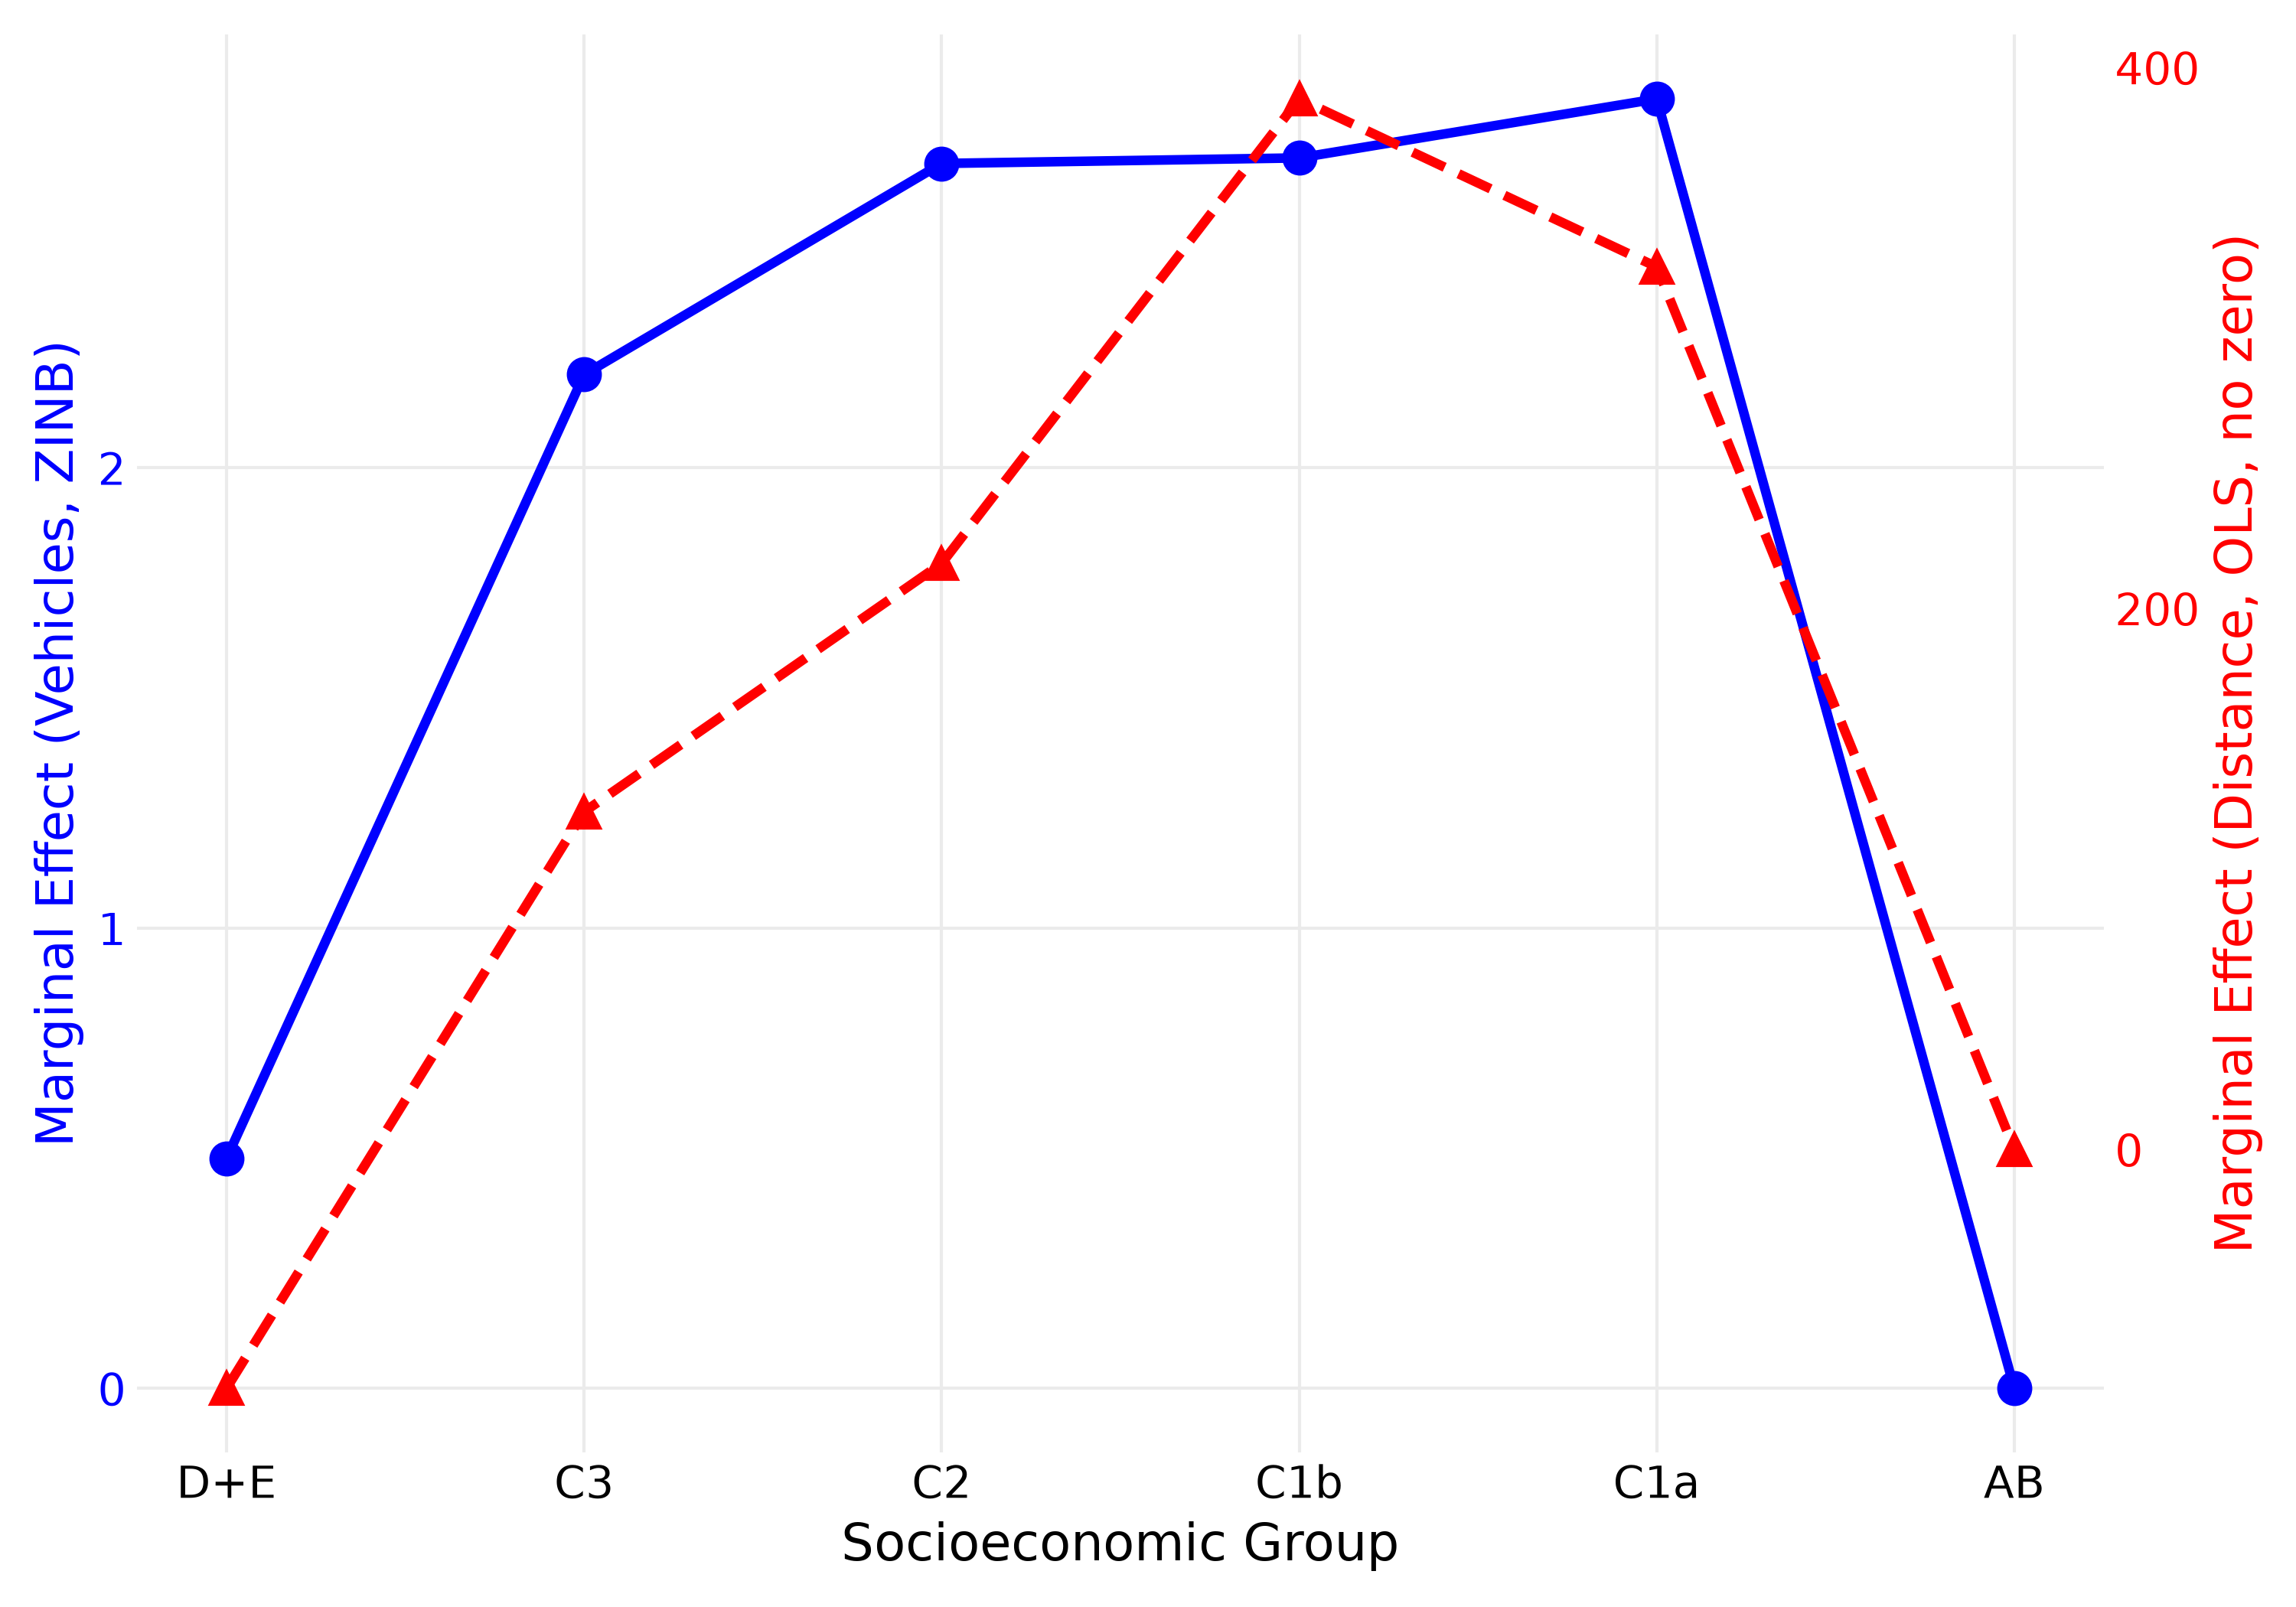
\includegraphics[width=\linewidth]{fig6_seg_dynamic.png}\\{\scriptsize Réplica}
  \end{columns}
  \vspace{2pt}
  {\footnotesize Mismos puntos (dif.\ $\le10^{-4}$). U invertida por GSE. El eje derecho está reescalado: comparan formas, no magnitudes.}
\end{frame}

\begin{frame}{Figura 8: efectos marginales por edad, modelo dinámico}
  \centering
  \begin{columns}[T]
    \column{0.49\textwidth}\centering
    \includegraphics[width=\linewidth]{Figura8_paperOriginal.png}\\{\scriptsize Paper (Fig.~8)}
    \column{0.49\textwidth}\centering
    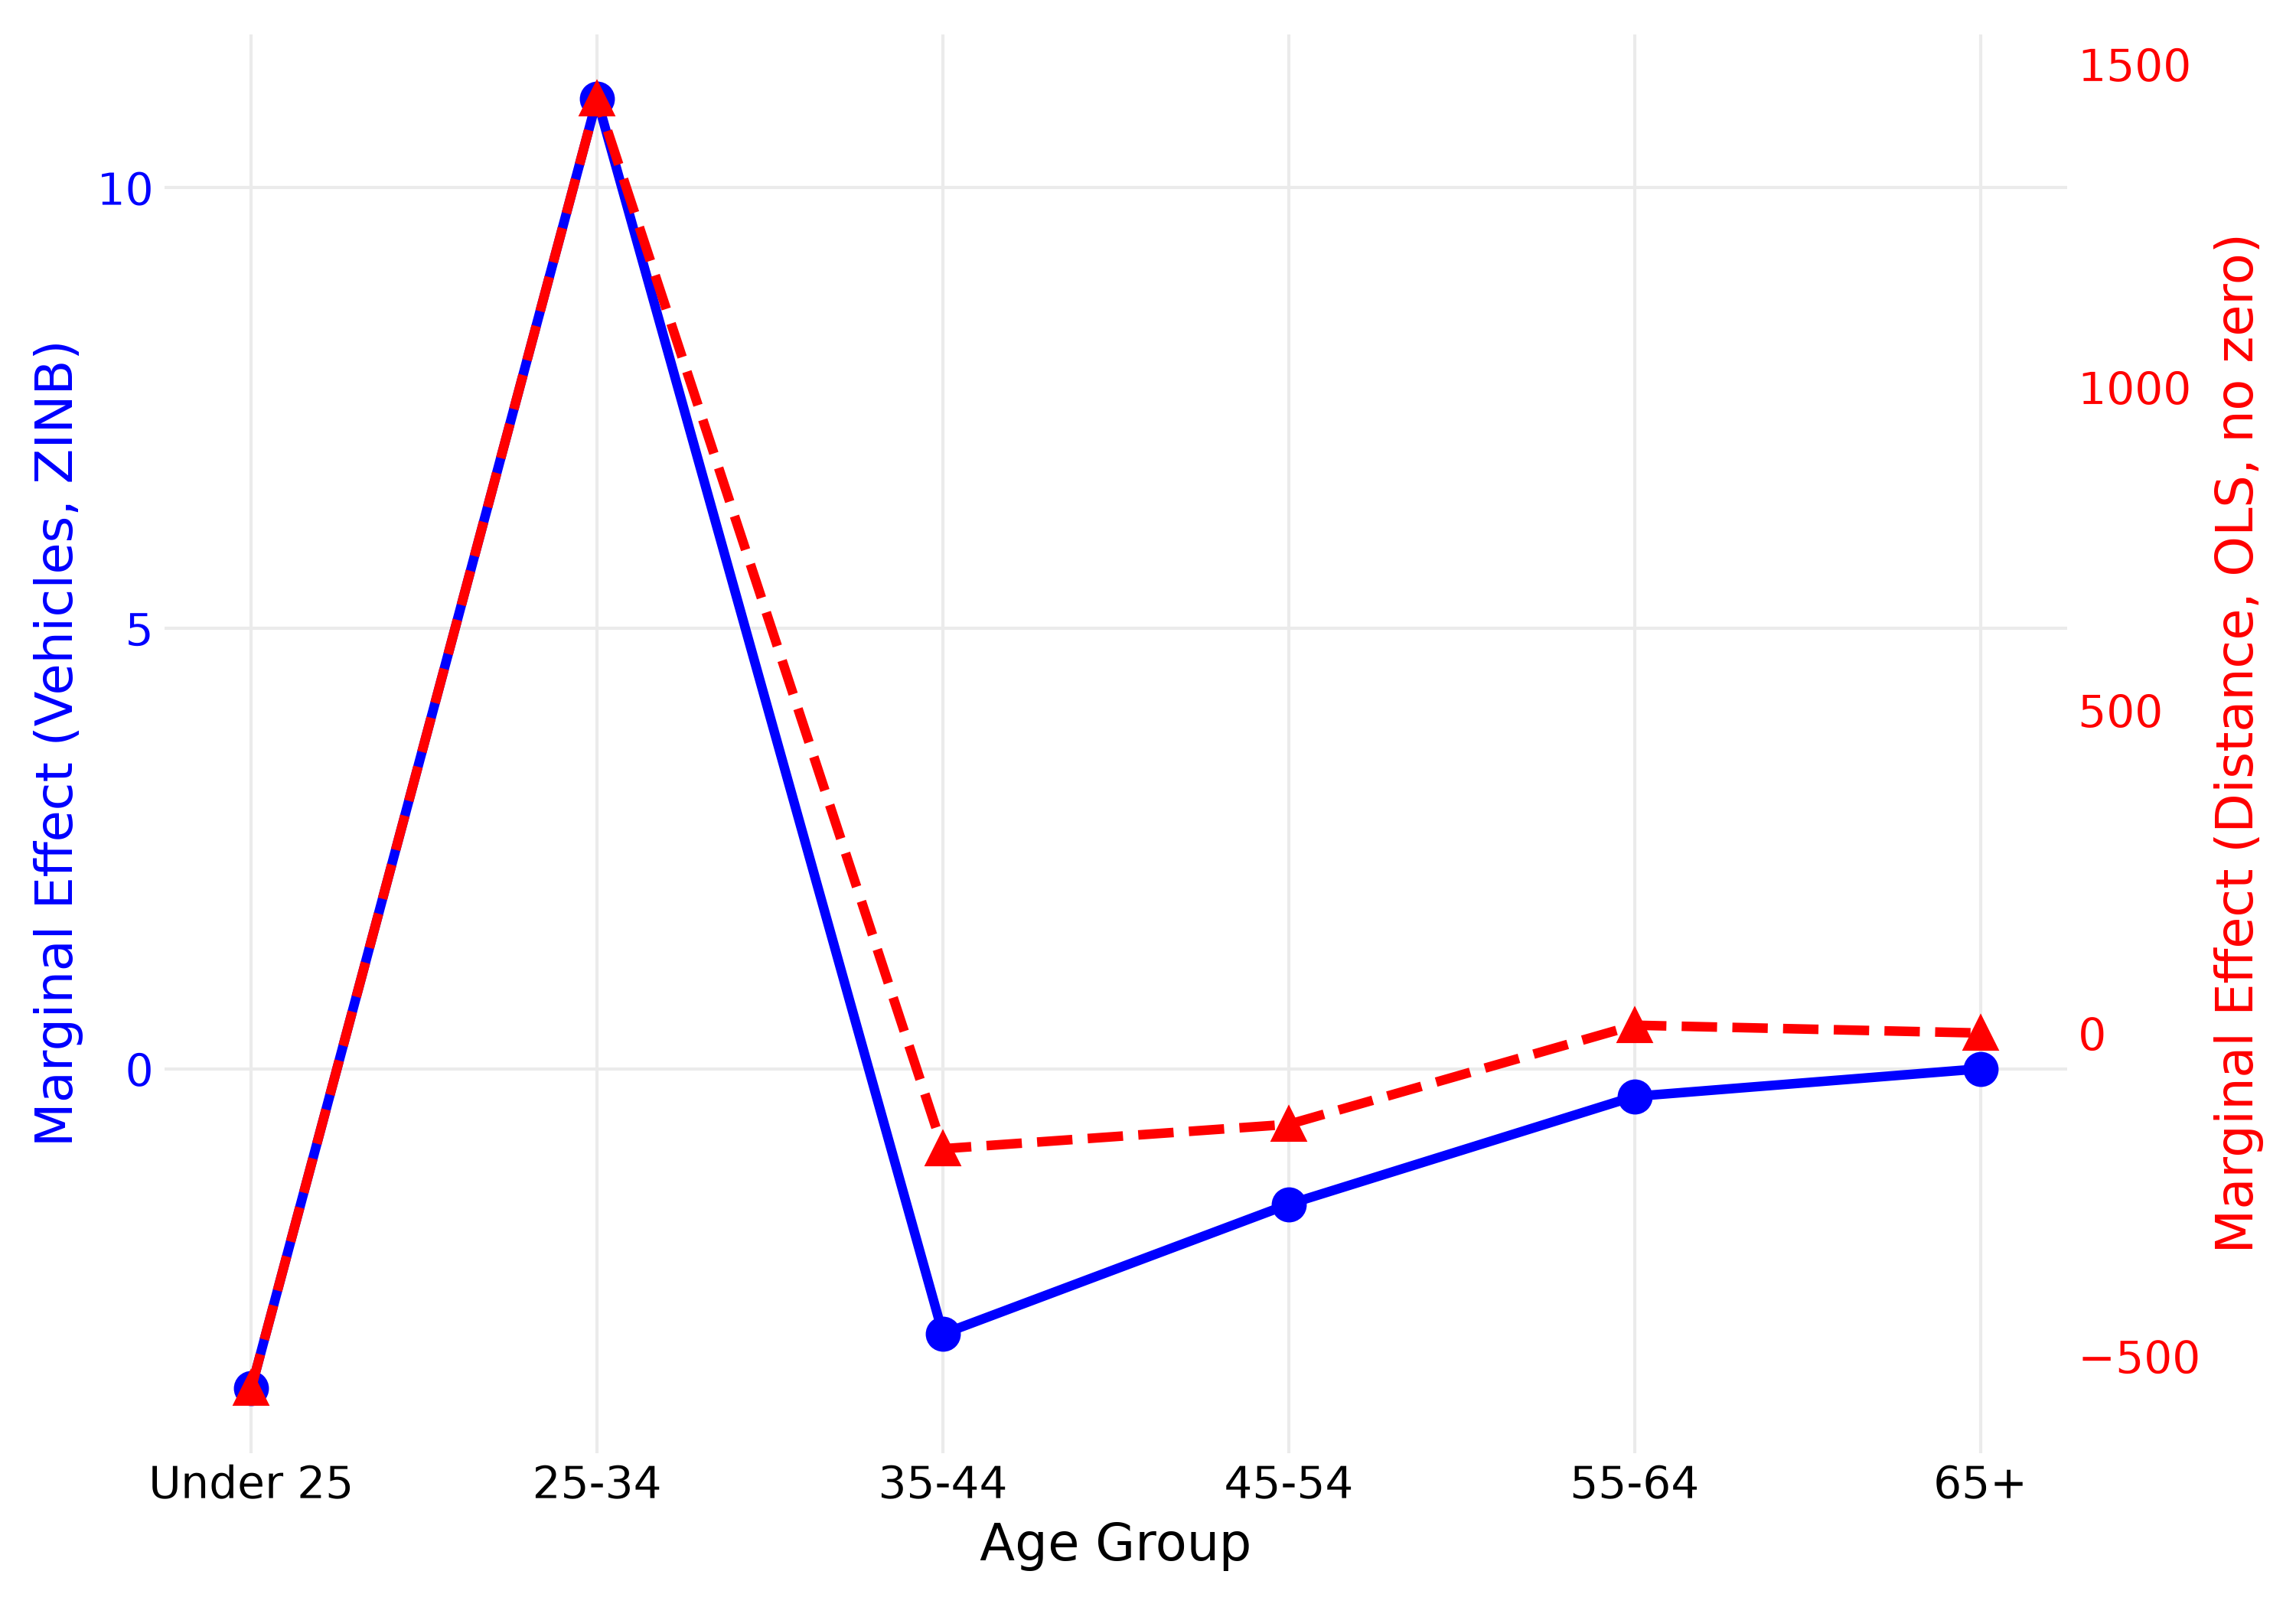
\includegraphics[width=\linewidth]{fig8_age_dynamic.png}\\{\scriptsize Réplica}
  \end{columns}
  \vspace{2pt}
  {\footnotesize Mismos puntos. Pico en 25--34 años; menores de 25 y mayores de 65 poco expuestos.}
\end{frame}

\begin{frame}{Figura 9: efectos marginales por GSE, modelo estático}
  \centering
  \begin{columns}[T]
    \column{0.49\textwidth}\centering
    \includegraphics[width=\linewidth]{Figura9_paperOriginal.png}\\{\scriptsize Paper (Fig.~9)}
    \column{0.49\textwidth}\centering
    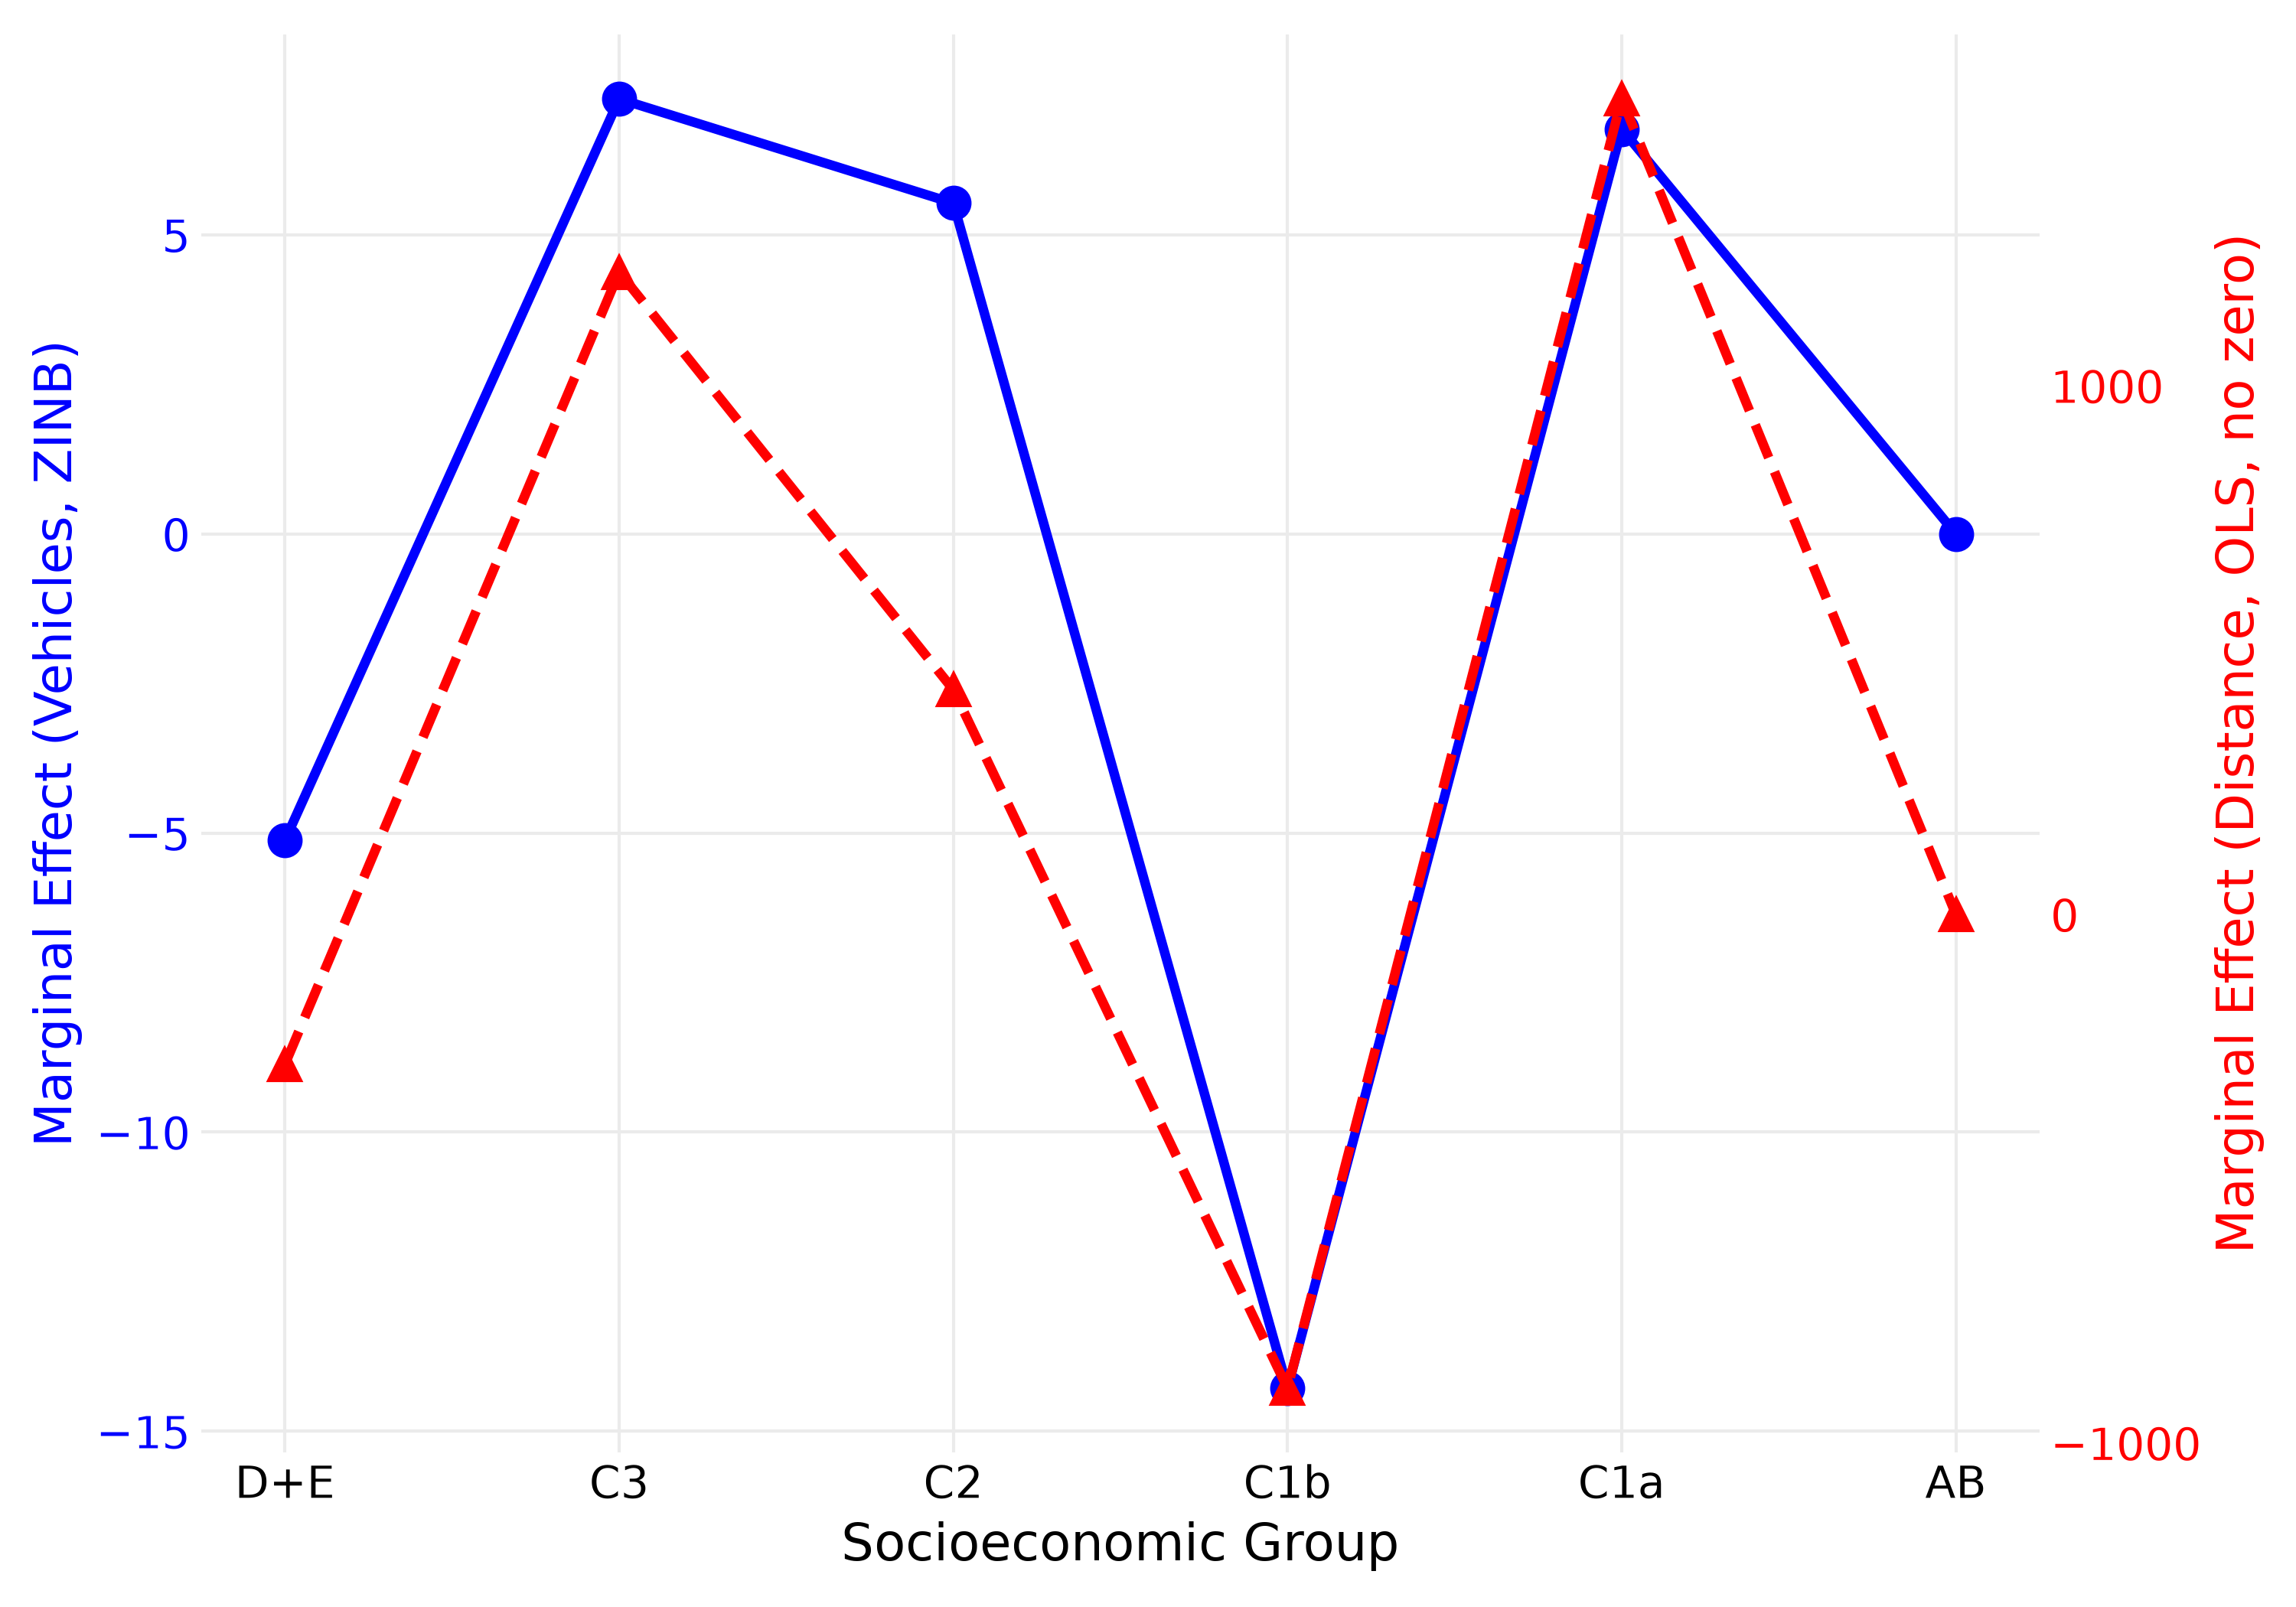
\includegraphics[width=\linewidth]{fig9_seg_static.png}\\{\scriptsize Réplica}
  \end{columns}
  \vspace{2pt}
  {\footnotesize Mismos puntos. En el enfoque estático C1b pasa a ser el menos expuesto en conteo (ZINB: $+2{,}67\to-14{,}28$).}
\end{frame}

\begin{frame}{Figura 10: efectos marginales por edad, modelo estático}
  \centering
  \begin{columns}[T]
    \column{0.49\textwidth}\centering
    \includegraphics[width=\linewidth]{Figura10_paperOriginal.png}\\{\scriptsize Paper (Fig.~10)}
    \column{0.49\textwidth}\centering
    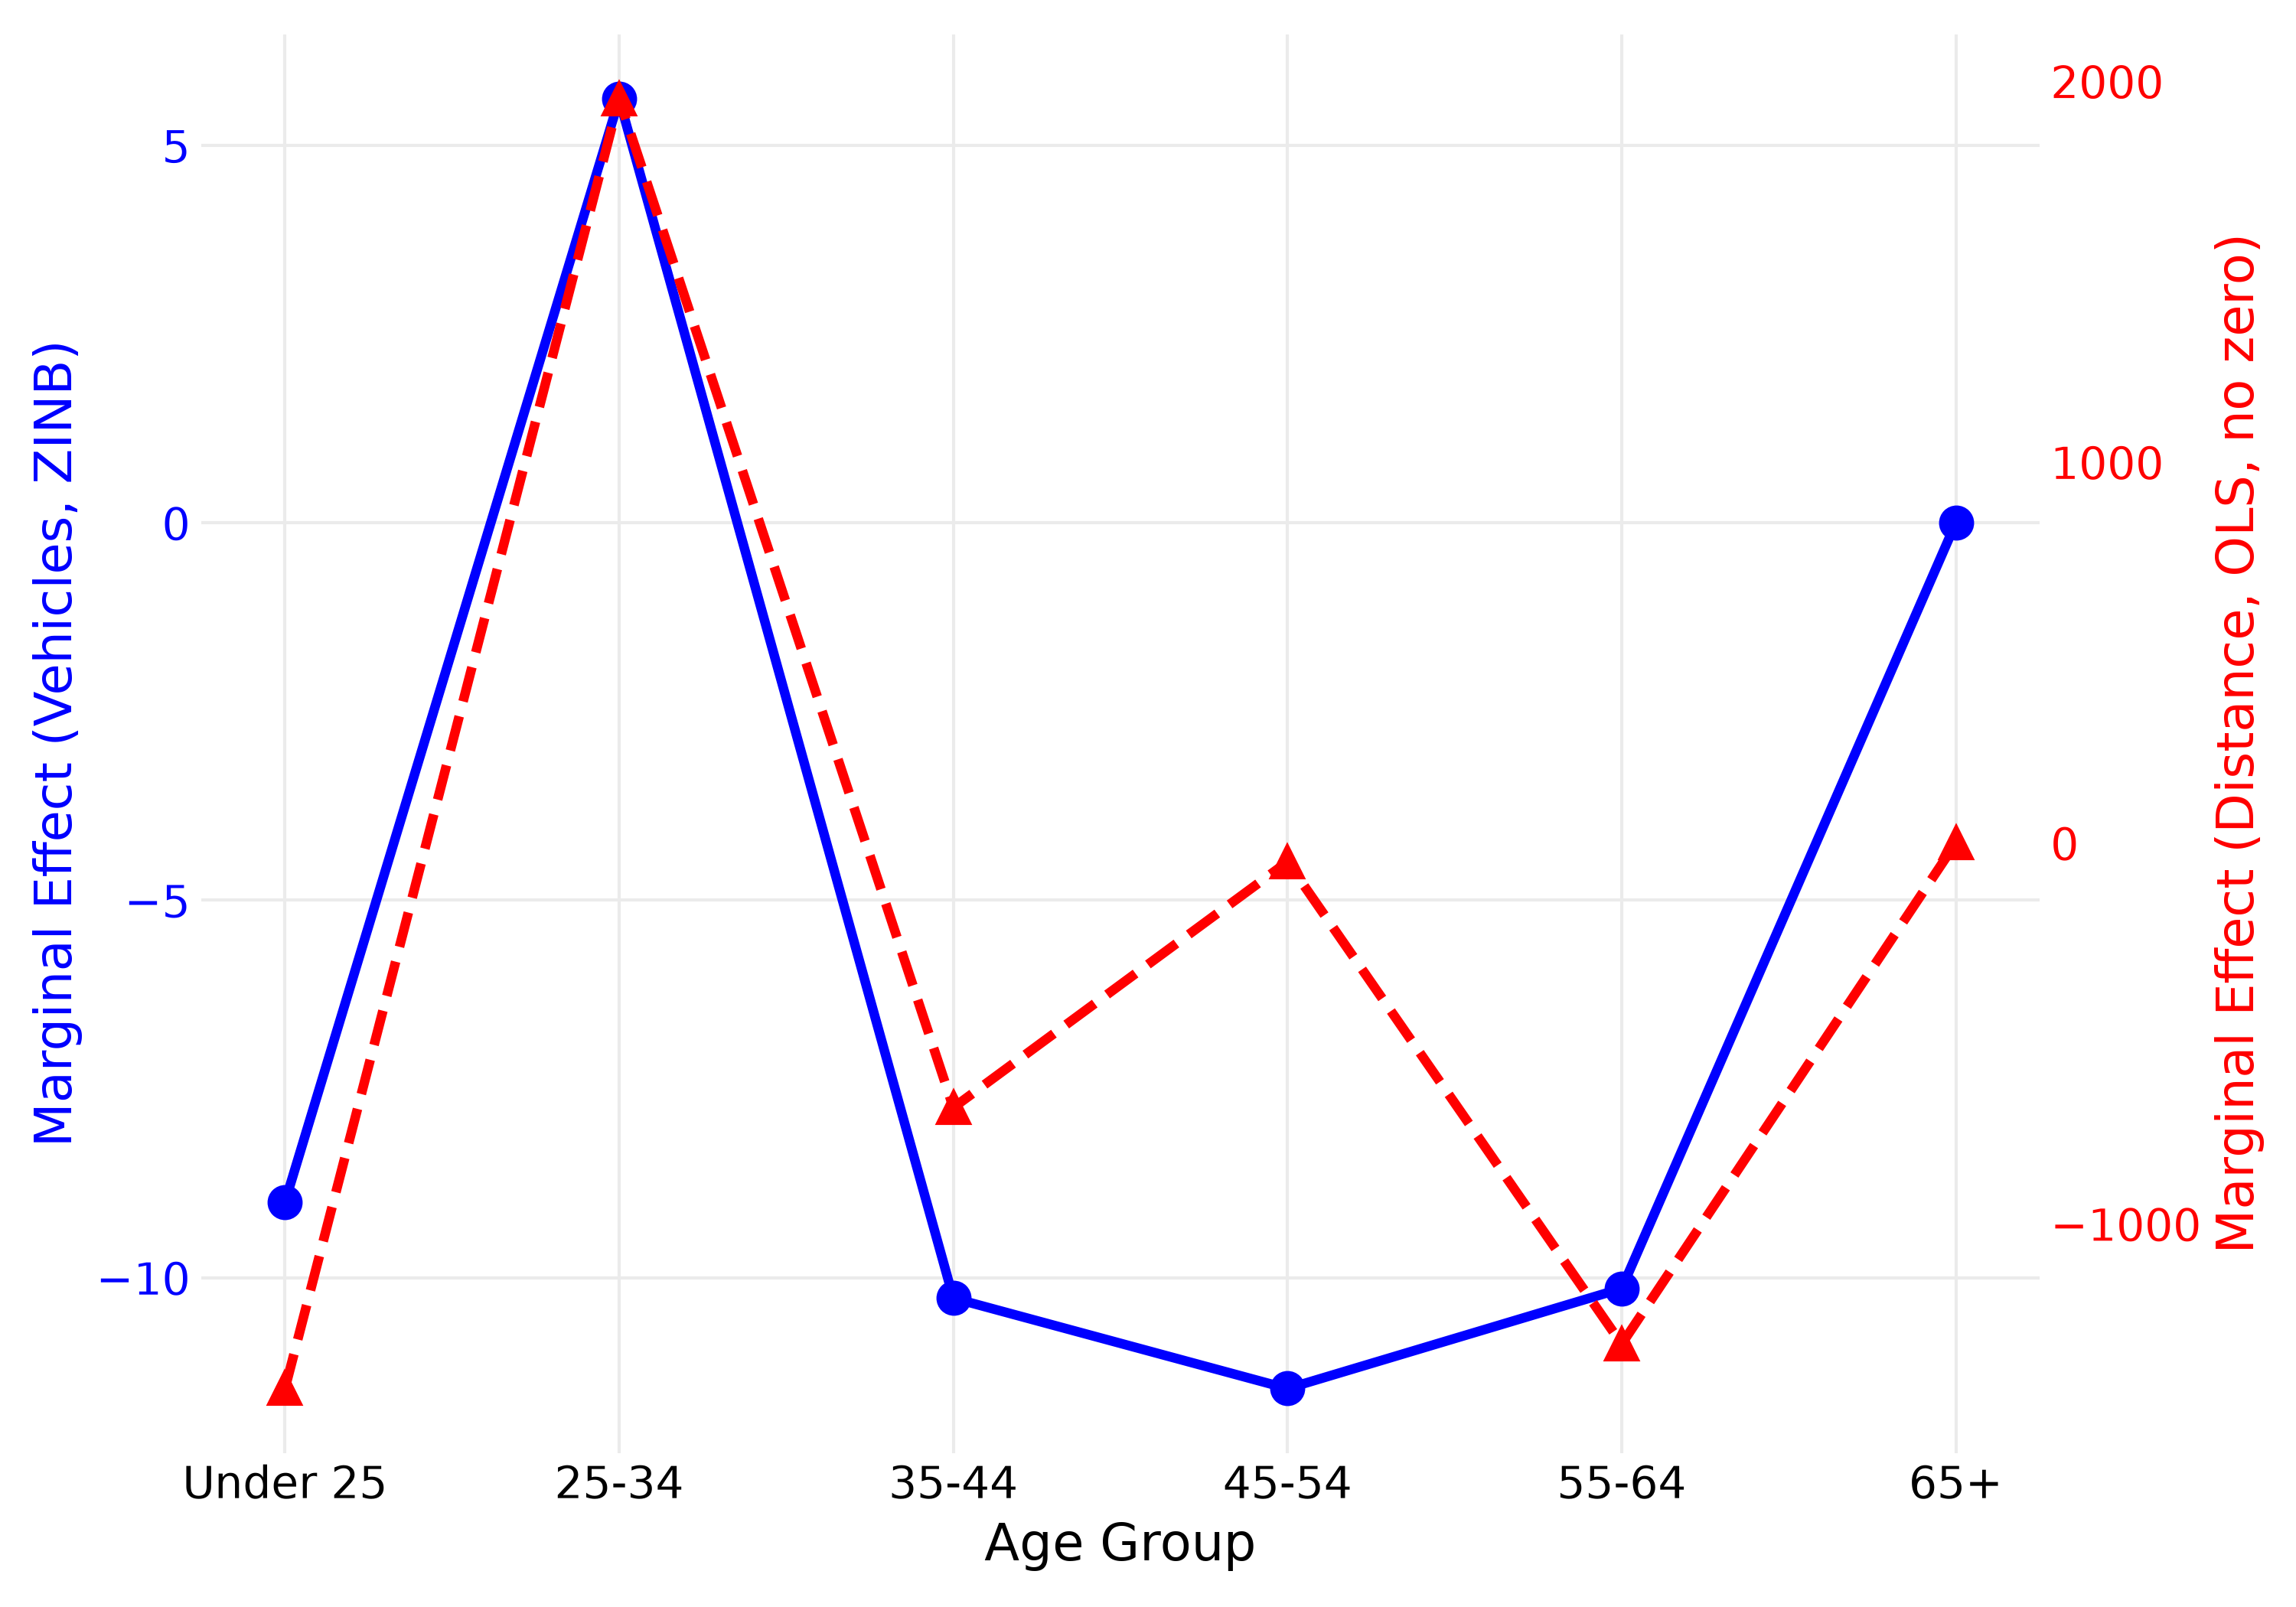
\includegraphics[width=\linewidth]{fig10_age_static.png}\\{\scriptsize Réplica}
  \end{columns}
  \vspace{2pt}
  {\footnotesize Mismos puntos (dif.\ $\le10^{-4}$). En el estático se mantiene el pico en 25--34 y los demás grupos quedan negativos en conteo.}
\end{frame}

\begin{frame}{Figura 7: gramos de NOx y PM por GSE}
  \centering
  \begin{columns}[T]
    \column{0.49\textwidth}\centering
    \includegraphics[width=\linewidth]{Figura7_paperOriginal.png}\\{\scriptsize Paper (Fig.~7)}
    \column{0.49\textwidth}\centering
    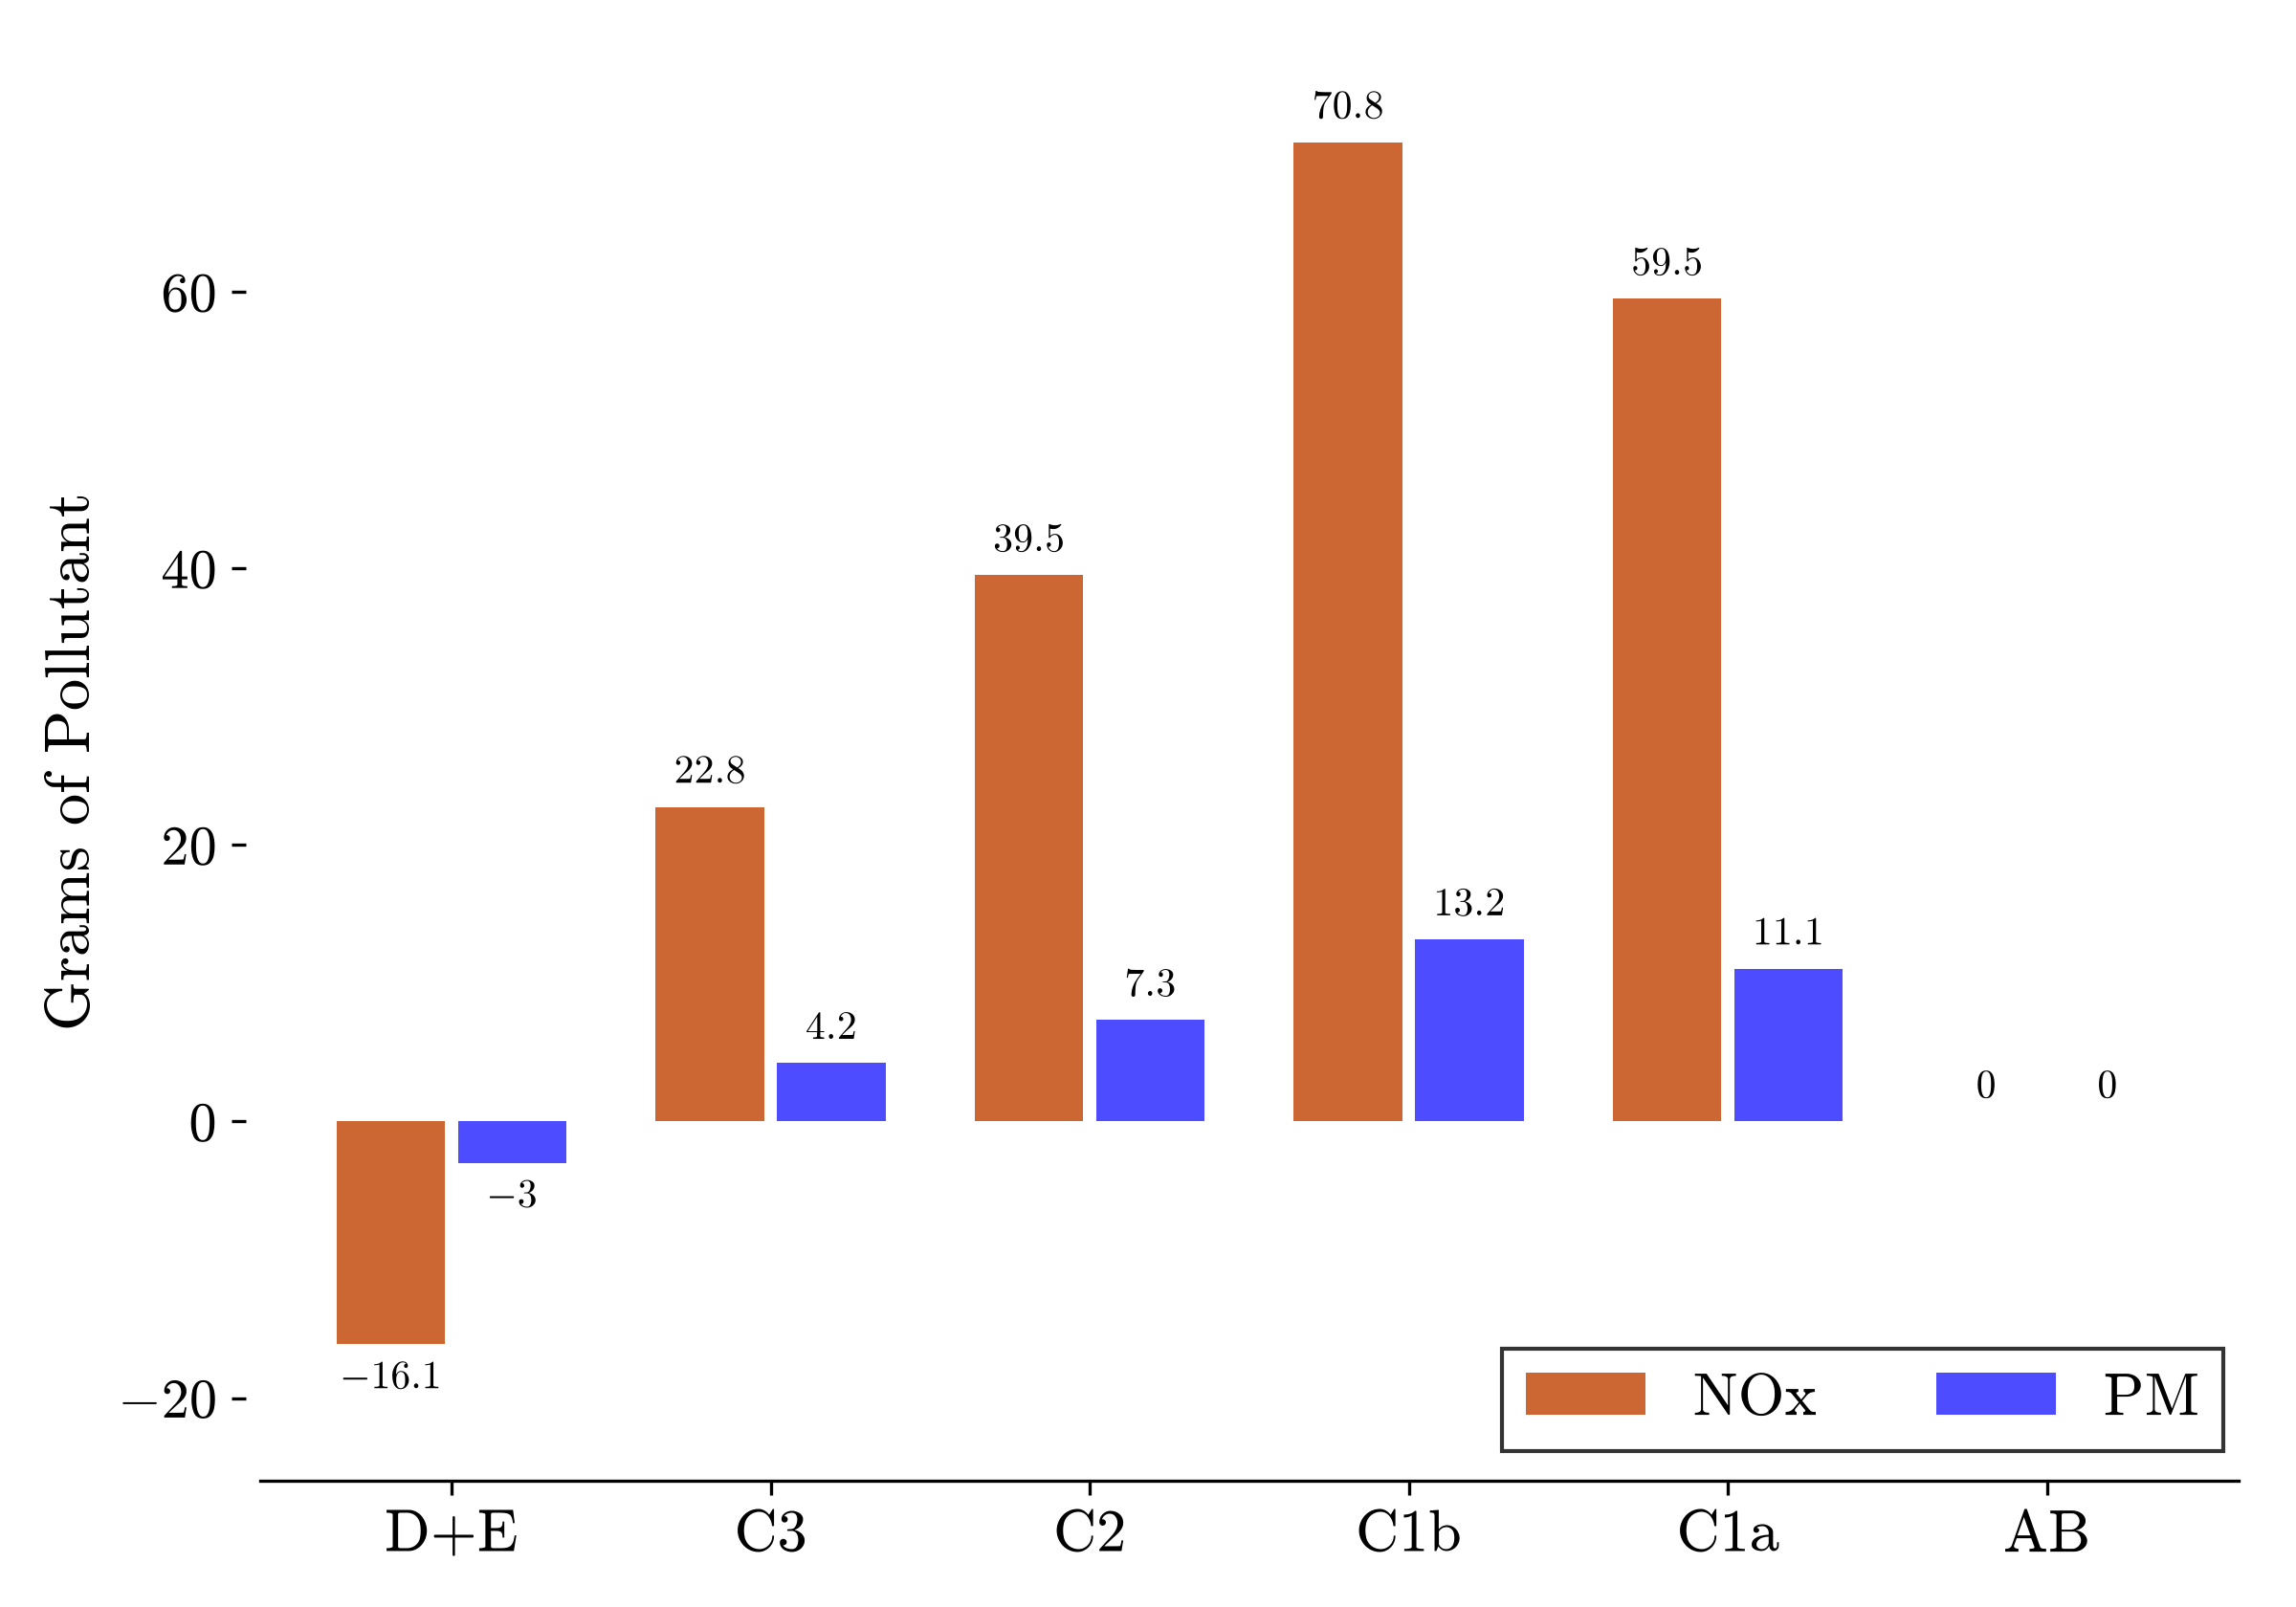
\includegraphics[width=\linewidth]{fig7_emissions_seg.png}\\{\scriptsize Réplica}
  \end{columns}
  \vspace{2pt}
  {\footnotesize Reproduce las 12 etiquetas, pero con factores \textbf{derivados de las propias barras} (0,182 g de NOx y 0,034 g de PM por metro marginal): no es una estimación independiente de emisiones.}
\end{frame}

\begin{frame}[plain]
  \centering
  \begin{columns}[T]
    \column{0.49\textwidth}\centering
    \includegraphics[height=7.2cm]{Figura1_paperOriginal.png}\\{\scriptsize Paper (Fig.~1)}
    \column{0.49\textwidth}\centering
    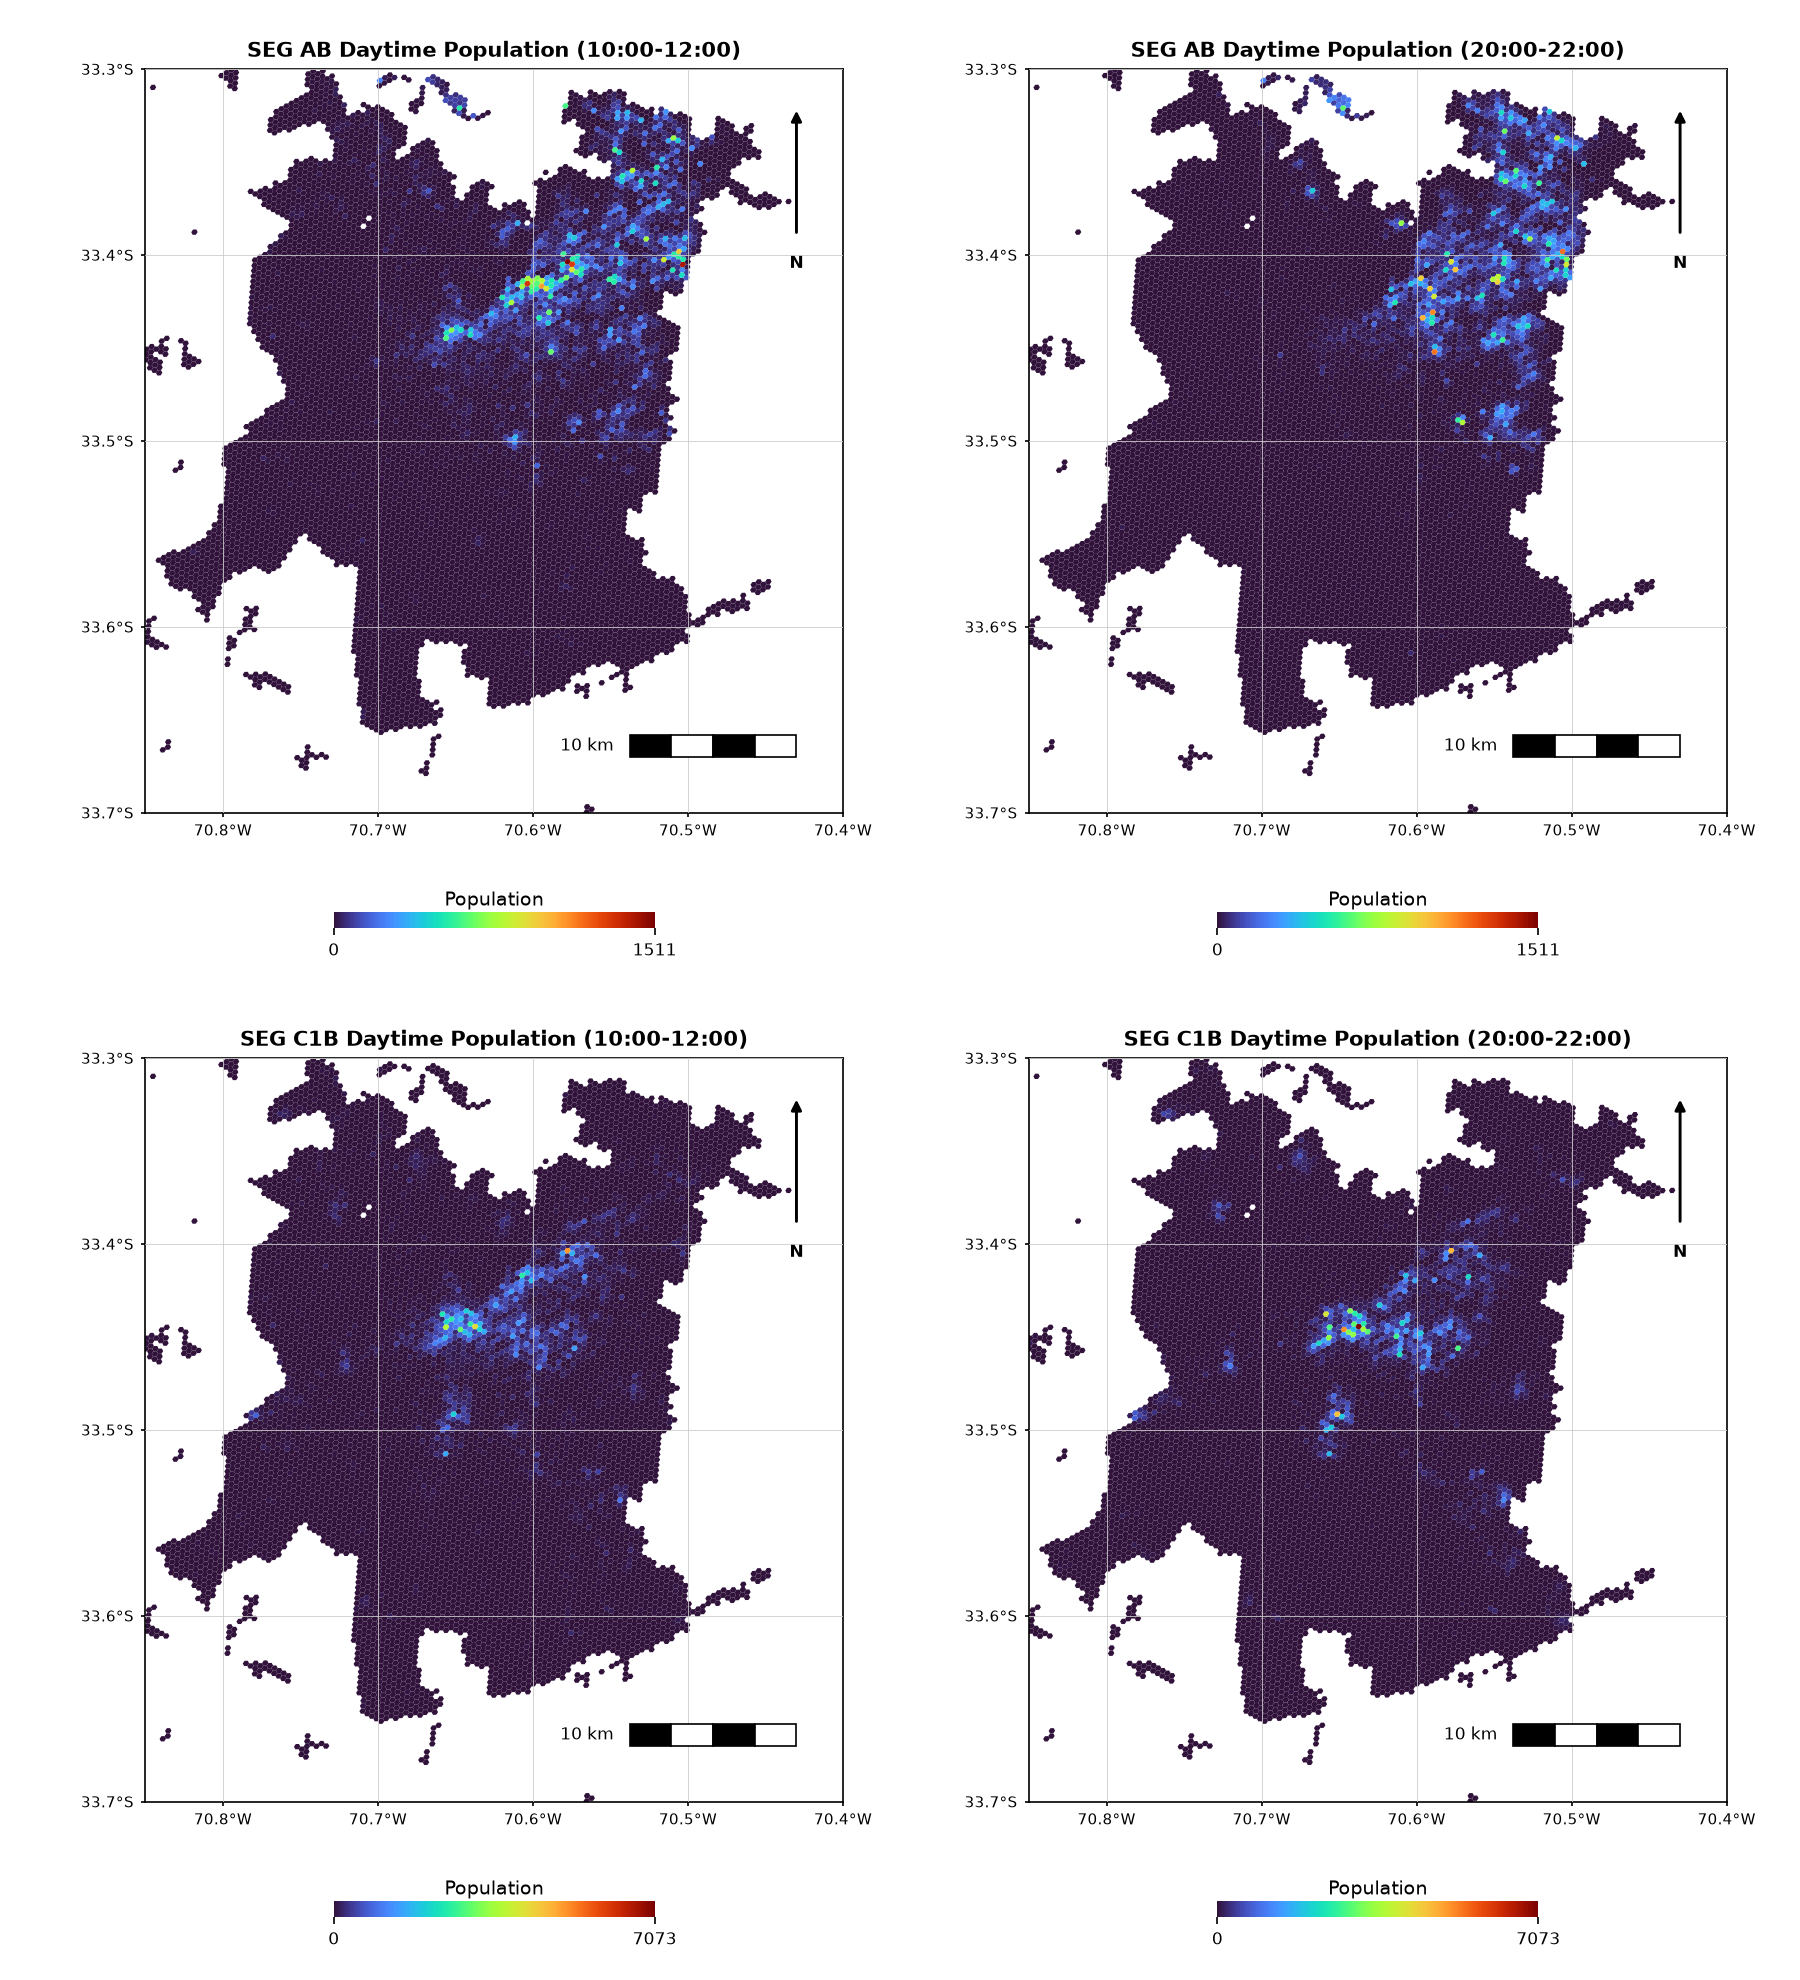
\includegraphics[height=7.2cm]{fig1_seg_population.png}\\{\scriptsize Réplica}
  \end{columns}
  {\scriptsize Fig.~1, población de AB y C1b por la mañana y por la tarde: el patrón se reproduce; la escala de color difiere (1.511 y 7.073 frente a 1.600 y 7.000).}
\end{frame}

\begin{frame}[plain]
  \centering
  \begin{columns}[T]
    \column{0.49\textwidth}\centering
    \includegraphics[height=7.2cm]{Figura2_paperOriginal.png}\\{\scriptsize Paper (Fig.~2): puntos GPS por hexágono}
    \column{0.49\textwidth}\centering
    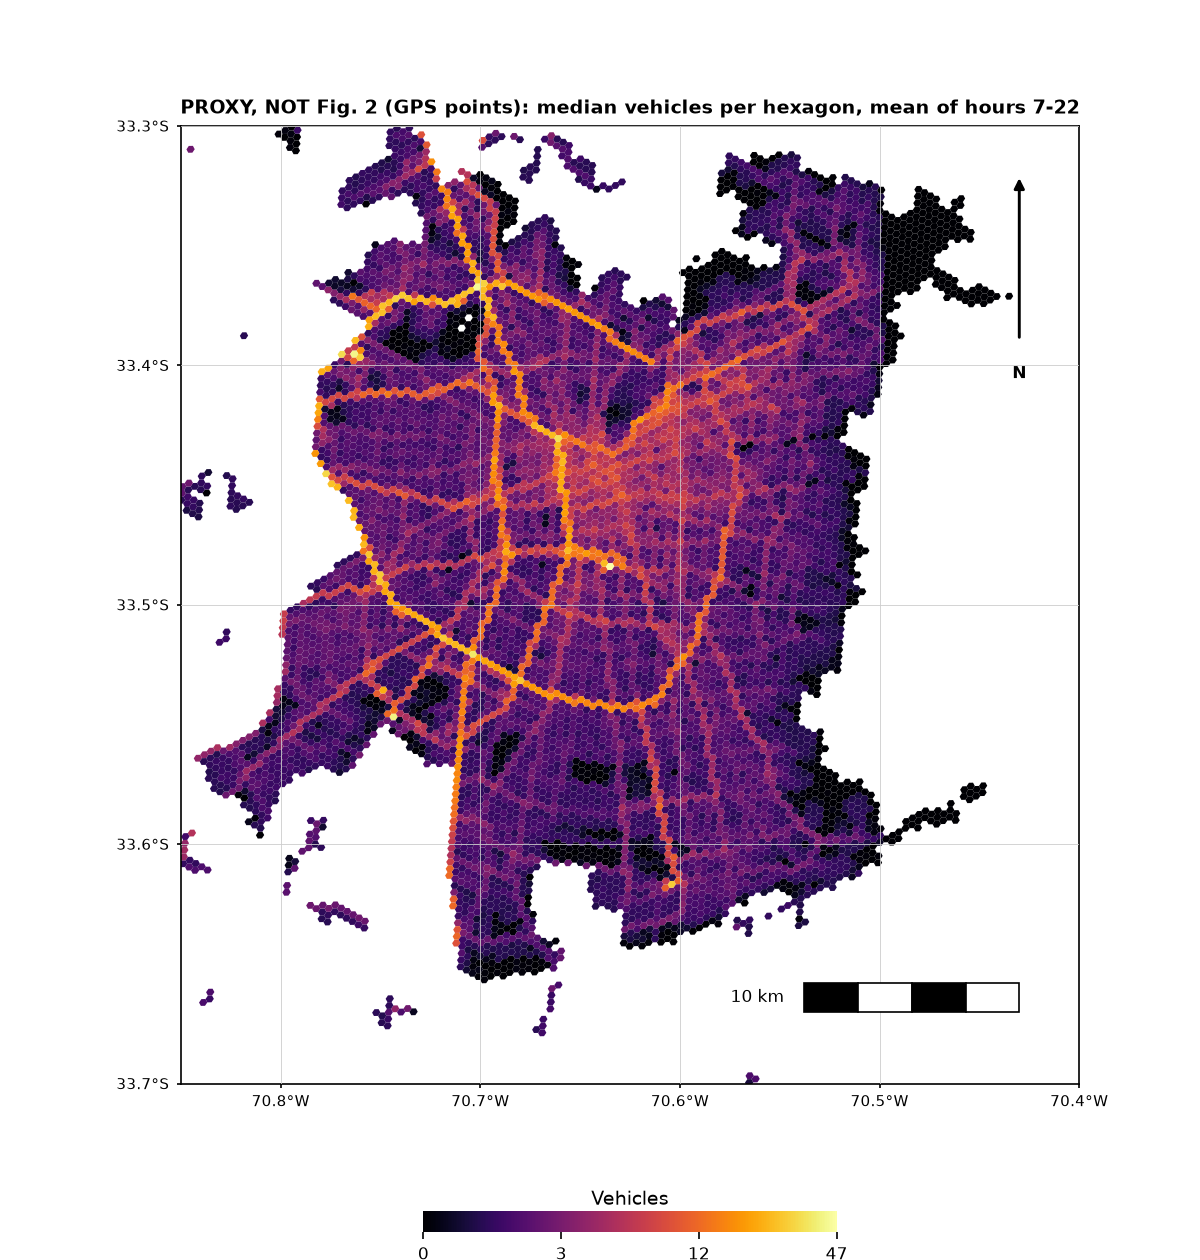
\includegraphics[height=7.2cm]{fig2_proxy_vehicles.png}\\{\scriptsize Sustituto rotulado (vehículos por hexágono)}
  \end{columns}
  {\scriptsize La Fig.~2 requiere el GPS crudo de todos los días, que no tenemos. El sustituto usa otra variable y no es una réplica.}
\end{frame}

% ------------------------------------------------------------------------------------------------
\section{Lo que difiere}

\begin{frame}{Estrellas: coincidencias y diferencias}
  \centering\small
  \begin{tabular}{lcc}\toprule
    Estrellas iguales entre\ldots & Tabla 4 (dinámica) & Tabla 5 (estática) \\\midrule
    Réplica y \textbf{tablas regeneradas por los autores} & \textbf{44/44} & \textbf{44/44} \\
    Réplica e \textbf{impresas en el paper} & 23/44 & 38/44 \\
    Autores (regeneradas) e impresas & 23/44 & 38/44 \\\bottomrule
  \end{tabular}

  \vspace{6pt}
  \begin{flushleft}\footnotesize
    \begin{itemize}
      \item Nuestro cálculo coincide con el de los autores en las 88 celdas. Lo que no coincide es lo \textbf{impreso}, y tampoco coincide con su propio código.
      \item \textbf{Se reconoce}: Dicen que parecen venir de una corrida distinta. Hipótesis es que se usó por error una base de prueba de 2 miércoles.
      \item Réplica de la Tabla 5: (ZINB sin agrupar). Con cluster por comuna en todo, coincide 27/44 con lo impreso.
    \end{itemize}
  \end{flushleft}
\end{frame}

\begin{frame}{Estrellas: dónde difieren (Tabla 4)}
  \centering\small
  \begin{tabular}{lcc}\toprule
    Celda & Réplica & Impreso \\\midrule
    Hombre, OLS & $\cdot$ & $*$ \\
    Hombre, OLS $\tilde K>0$ & $**$ & $***$ \\
    35--44 años, OLS $\tilde K>0$ & ninguna & $***$ \\
    Hombre, Log OLS (el ``24\,\%'') & ninguna & $***$ \\
    45--54 años, Log OLS & $***$ & ninguna \\
    C1b, ZINB & $*$ & ninguna \\\bottomrule
  \end{tabular}

  \vspace{6pt}
  \begin{flushleft}\footnotesize
    \begin{itemize}
      \item De las 21 celdas distintas, en \textbf{17} la réplica tiene \emph{menos} estrellas: lo publicado aparenta más significancia de la que da el método.
      \item Las diferencias no tocan los \textbf{valores} (signo y magnitud), que son lo que dibujan las figuras.
    \end{itemize}
  \end{flushleft}
\end{frame}

\begin{frame}{Estrellas: el ZINB estático y el cluster \texttt{NULL}}
  \begin{itemize}
    \item En el script estático de los autores la variable del cluster queda vacía (\texttt{NULL}): cada fila es su propio cluster, es decir, errores \textbf{sin agrupar}.
  \end{itemize}
  \centering\small
  \begin{tabular}{lc}\toprule
    Cluster del ZINB estático & Estrellas \\\midrule
    Sin agrupar (\texttt{NULL}, lo que imprime el paper) & 11/11 con $***$ \\
    Por comuna (lo que dice el paper) & 4/11 con alguna estrella y ninguna $***$ \\\bottomrule
  \end{tabular}

  \vspace{6pt}
  \begin{flushleft}\footnotesize
    \begin{itemize}
      \item Con cluster por comuna, el C1b estático (ZINB $-14{,}28$) no se distingue de cero ($p\approx0{,}48$): la diferencia dinámico--estático de C1b solo es significativa con el cluster que el script omite.
      \item Los autores no mencionaron este punto; está entre las consultas de la segunda ronda.
    \end{itemize}
  \end{flushleft}
\end{frame}

\begin{frame}{I de Moran: no se reproduce}
  \centering\footnotesize
  \begin{tabular}{lrr}\toprule
Lectura (anillo 1 de H3) & Distancia & Vehículos \\\midrule
\textbf{promedio de las 16 I horarias (W)} & \textbf{0,419} & \textbf{0,430} \\
mapa promediado entre horas (W) & 0,466 & 0,470 \\
horas apiladas (W) & 0,462 & 0,466 \\
promedio de las 16 I horarias (B) & 0,427 & 0,440 \\
mapa promediado entre horas (B) & 0,472 & 0,479 \\
horas apiladas (B) & 0,473 & 0,477 \\
\midrule
\textbf{Paper} & \textbf{0,4694} & \textbf{0,4756} \\
\bottomrule\end{tabular}
\\[4pt]
  \begin{flushleft}\footnotesize
    \begin{itemize}
      \item El paper no define la matriz de pesos ni cómo promedia las 16 horas, y el paquete no trae explicación exacta del método. W: filas estandarizadas; B: binaria.
      \item La lectura literal da 0,419 y 0,430; las alternativas se acercan (a ~1--2\,\%) pero ninguna da el cuarto decimal.
      \item Todas las lecturas dan $I\gg0$: la \textbf{correlación espacial positiva se confirma.}
    \end{itemize}
  \end{flushleft}
\end{frame}

\begin{frame}{Wasserstein (movilidad, Tabla 2): 13 de 15 dentro de la banda}
  \centering\scriptsize
  \begin{columns}[T]
    \column{0.52\textwidth}\centering\begin{tabular}{lrrcc}\toprule
Grupo & Impreso & Mediana & Banda 95\,\% & ¿Dentro? \\\midrule
Male & 1,024 & 1,027 & 1,017--1,038 & sí \\
Female & 0,976 & 0,973 & 0,962--0,983 & sí \\
Under 25 & 0,920 & 0,943 & 0,903--0,986 & sí \\
25-34 & 0,998 & 0,989 & 0,967--1,015 & sí \\
35-44 & 1,002 & 1,014 & 0,991--1,040 & sí \\
45-54 & 1,122 & 1,100 & 1,049--1,148 & sí \\
55-64 & 1,055 & 1,025 & 0,988--1,086 & sí \\
65+ & 0,726 & 0,706 & 0,672--0,759 & sí \\
\bottomrule\end{tabular}

    \column{0.46\textwidth}\centering\begin{tabular}{lrrcc}\toprule
Grupo & Impreso & Mediana & Banda 95\,\% & ¿Dentro? \\\midrule
AB & 1,337 & 1,246 & 1,070--1,476 & sí \\
C1a & 0,604 & 0,566 & 0,467--0,667 & sí \\
C1b & 0,508 & 0,463 & 0,386--0,556 & sí \\
C2 & 1,000 & 0,888 & 0,749--1,000 & sí \\
C3 & 1,066 & 1,011 & 1,000--1,110 & sí \\
D & 0,968 & 1,019 & 1,000--1,104 & \textbf{no} \\
E & 1,157 & 1,023 & 0,989--1,138 & \textbf{no} \\
\bottomrule\end{tabular}

  \end{columns}
  \vspace{4pt}
  \begin{flushleft}\footnotesize
    \begin{itemize}
      \item Los autores calculan el valor con una \textbf{muestra aleatoria de 5.000 hexágonos sin semilla}: lo impreso es una sola extracción. Se replicó el método con 200 semillas.
      \item Estable: hombre $>$ mujer; 45--54 el más móvil y 65+ el menos; AB el más móvil y C1b el menos. No estable: el orden de C2, C3, D y E.
    \end{itemize}
  \end{flushleft}
\end{frame}

\begin{frame}{Otras diferencias}
  \centering\footnotesize
  \setlength{\tabcolsep}{4pt}
  \begin{tabular}{p{2.3cm}p{2.7cm}p{2.9cm}p{4.6cm}}\toprule
    Ítem & Paper & Réplica & Motivo \\\midrule
    Fig.~1, escala (AB) & 1.600 & 1.511 & Se desconoce; hipótesis: otro período o versión del panel \\
    Fig.~1, escala (C1b) & 7.000 & 7.073 & Ídem \\
    Fig.~7 & 12 etiquetas & 12/12 & Factor derivado de las propias barras \\
    Fig.~2 & Puntos GPS por hexágono & Sustituto & Falta el GPS crudo \\
  \end{tabular}
\end{frame}

% ------------------------------------------------------------------------------------------------
\section{Lo que difiere en el original}

\begin{frame}{Donde el paper o su código difieren de lo que dicen}
  \centering\scriptsize
  \begin{tabular}{p{5.2cm}p{5.4cm}p{1.9cm}}\toprule
    Qué ocurre & Qué hicimos & Hallazgo \\\midrule
    Hora UTC en los camiones y hora local en la población (desfase de 3--4 h; los autores lo reconocen) & Replicamos tal cual y agregamos una sensibilidad en hora local & H1, H33 \\
    La mediana omite los días sin vehículos (no los cuenta como 0) & Replicamos el código; la variante con ceros cambia el 41\,\% de las filas & H2 \\
    La distancia descarta los tramos que cruzan hexágono u hora (el paper dice recortar) & Replicamos el código & H4 \\
    ``OLS $\tilde K>0$'' es un modelo de dos partes (logit + OLS) & Replicado así; un OLS simple da otras cifras & H7 \\
    La columna ``ZINB'' es la binomial negativa ($\hat\pi=0$) & Se reporta el máximo de la verosimilitud & H23, H29 \\
    $(1-\pi)$ se aplica dos veces en el efecto marginal & Documentado; no afecta porque $\hat\pi=0$ & H10 \\
    El ``24\,\% de hombres'' viene del modelo log y no es significativo & Documentado; los autores coinciden & H31, H32 \\\bottomrule
  \end{tabular}
\end{frame}

\begin{frame}{Sensibilidad con la hora local (aporte propio)}
  \begin{itemize}
    \item Camiones convertidos a \texttt{America/Santiago}; horas locales 7--19 (las únicas completas). Se compara con la versión publicada restringida a las mismas horas.
    \item \textbf{Las cuatro conclusiones del paper se mantienen.} Todos los cambios de signo ocurren en celdas no significativas en ambas versiones.
  \end{itemize}
  \centering\scriptsize
  \begin{tabular}{lccc}\toprule
    Modelo (tabla dinámica) & Cambios de signo & Cambios de estrellas & Cambio relativo mediano \\\midrule
    ZINB & 1 & 1 & 8\,\% \\
    OLS & 1 & 1 & 12\,\% \\
    OLS $\tilde K>0$ & 1 & 2 & 9\,\% \\
    Log OLS & 0 & 6 & 32\,\% \\\bottomrule
  \end{tabular}\\[2pt]
  \footnotesize 11 celdas por columna. El modelo log es el más sensible.
\end{frame}

% ------------------------------------------------------------------------------------------------
\section{Conclusiones}

\begin{frame}{¿Se confirman las conclusiones del paper?}
  \centering\scriptsize
  \begin{tabular}{p{3.7cm}p{2.3cm}p{2.0cm}p{4.3cm}}\toprule
    Conclusión & Figuras (mismos valores) & Hora corregida & Respaldo estadístico (cluster por comuna) \\\midrule
    \textbf{U invertida por GSE} & Sí & Se mantiene & Sí: $***$ en OLS $\tilde K>0$ para C1a, C1b, C2 y C3 \\
    \textbf{Pico en 25--34 años} & Sí & Se mantiene & Sí: $***$ en ZINB y OLS $\tilde K>0$ \\
    \textbf{C1b: de más expuesto (dinámico) a menos (estático)} & Sí en los puntos & Se mantiene & \textbf{Débil}: no significativo en el estático \\
    \textbf{Hombres 24\,\% más expuestos} & No aparece & --- & \textbf{No se sostiene} ($p=0{,}116$) \\\bottomrule
  \end{tabular}
  \vspace{4pt}

  \footnotesize Las desviaciones son del original (hora, base de las estrellas, cluster), no de nuestra implementación: los coeficientes coinciden con los publicados.
\end{frame}

\begin{frame}{Qué se puede y qué no se puede decir}
  \begin{columns}[T]
    \column{0.5\textwidth}
    \textbf{Se puede decir}
    \footnotesize
    \begin{itemize}
      \item Las celdas con más clase media (C1a a C3) y más gente de 25--34 años tienen más actividad de reparto.
      \item Medir la población presente en lugar de la residencial cambia el diagnóstico en C1b y en sexo.
      \item Esto se mantiene al corregir la hora.
    \end{itemize}
    \column{0.48\textwidth}
    \textbf{No se puede decir}
    \footnotesize
    \begin{itemize}
      \item Que una persona de C1b ``recibe X gramos más'': el análisis es ecológico, correlacional y de co-ocurrencia.
      \item Que los hombres están 24\,\% más expuestos.
      \item Que todas las estrellas impresas son correctas.
      \item Que la altura relativa de las dos líneas de una figura sea comparable (eje reescalado).
    \end{itemize}
  \end{columns}
  \vspace{6pt}

  \textbf{Pendiente} \footnotesize: respuesta de los autores a la segunda ronda (I de Moran, muestra del Wasserstein, cluster \texttt{NULL}, columna ``ZINB'' = NB y hora local de la población).
\end{frame}

\begin{frame}{Referencias}
  \footnotesize
  \vspace{6pt}
  \printbibliography
\end{frame}

\end{document}
